\documentclass{ximera}

\input{../preamble.tex}


\title{Comparing decimals}
\author{Jenny Sheldon}

\begin{document}

\begin{abstract}
We compare decimal numbers.
\end{abstract}
\maketitle

\section{Activities for this section:} 
%\link[The Decimal System]{https://ximera.osu.edu/m4t/elementaryActivities/SemesterOnePacket/elementaryActivities/Numbers/DecimalSystem}, 
\link[Comparing Decimals]{https://ximera.osu.edu/m4t/elementaryActivities/SemesterOnePacket/elementaryActivities/Numbers/ComparingDecimalsCards}

\vskip 0.2in

Now that we have represented decimal numbers using bundling, paper strips, and number lines, we will use each of these representations to decide which decimal number is larger. Throughout this section, pay attention to the ways that each representation shows the structure of the base-ten system, and write notes on how you would connect each representation back to the basic ideas of bundling.


\section{Comparing with bundling}


Let's jump right in to see how bundling can help us determine which of two decimal numbers is larger.

\begin{question}
Which is larger, $0.4$ or $0.39$?

\begin{explanation}
Start by noticing that while you probably already know the answer to this question, it can be tricky for kids. Visually $0.39$ looks longer because it has more digits. Does that mean it's the larger number? Drawing pictures of bundled objects will help us out here.

First, when we were comparing fractions, we made a big deal about how we couldn't compare fractions until our wholes were the same. When we compare decimals, the idea of the wholes being the same is identical to needing the value of one stick to be the same in each picture that we draw. We can't compare these numbers if we choose the value of one stick to be $0.1$ in the first number and $0.01$ in the second number. Let's choose to let the value of one stick be $0.01$ in this picture, because then we can represent both numbers without having to cut our sticks into ministicks. (There's absolutely nothing wrong with going the other direction. Maybe you can try out that version in your notes!)

Since we are taking one stick to be $0.01$, we know that one bundle has to have the value $\answer[given]{0.1}$. This is because when we bundle our sticks, we always write the number of bundles exactly one place to the left of the number of sticks. So, to represent $0.39$, we will need $\answer[given]{9}$ individual sticks and $\answer[given]{3}$ bundles. 

\begin{image}
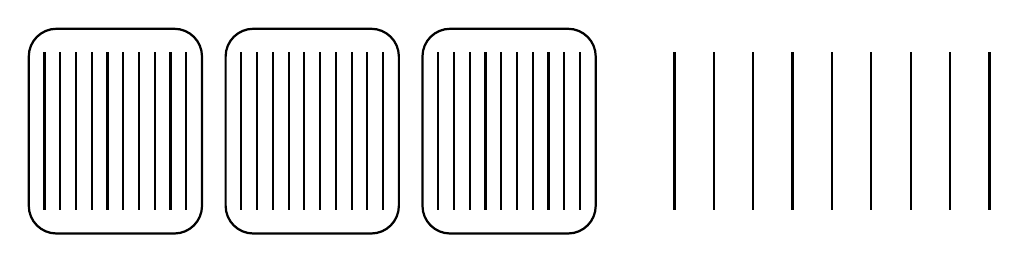
\begin{tikzpicture}
  % Parameters
  \def\stickheight{2}
  \def\stickgap{0.2}
  \def\ovalpad{0.2}
  \def\bundleSpacing{2.5} % narrower bundle spacing
  \def\stickSpacing{0.5}  % narrower stick spacing

  % Define bundle drawing as a TikZ pic
  \tikzset{
    bundle/.pic={
      % Draw 10 sticks
      \foreach \i in {0,...,9} {
        \draw[thick] (\i*\stickgap,0) -- (\i*\stickgap,\stickheight);
      }
      % Oval around bundle
      \draw[thick, rounded corners=10pt]
        (-\ovalpad, -0.3) rectangle (9*\stickgap+\ovalpad, \stickheight+0.3);
    }
  }

  % Draw 3 bundles
  \foreach \i in {0,...,2} {
    \begin{scope}[shift={(\i*\bundleSpacing,0)}]
      \pic{bundle};
    \end{scope}
  }

  % Draw 9 sticks, starting after the last bundle
  \pgfmathsetmacro{\startX}{3*\bundleSpacing + 0.5} % 0.5 unit gap after last bundle
  \foreach \i in {0,...,8} {
    \draw[thick]
      ({\startX + \i*\stickSpacing}, 0) -- ({\startX + \i*\stickSpacing}, \stickheight);
  }

\end{tikzpicture}
\end{image}

Drawing $0.4$ could be a bit more confusing. But notice that we don't have anything in the $0.01$ place, so we can also write this number as $0.40$. Notice that the $4$ is still in the tenths place, and the zero in the hundredths place means we have no objects in that place, so we didn't change the value of this number at all. When we write the number as $0.40$, we can see that in order to represent this number, we will need $\answer[given]{0}$ individual sticks and $\answer[given]{4}$ bundles.

\begin{image}
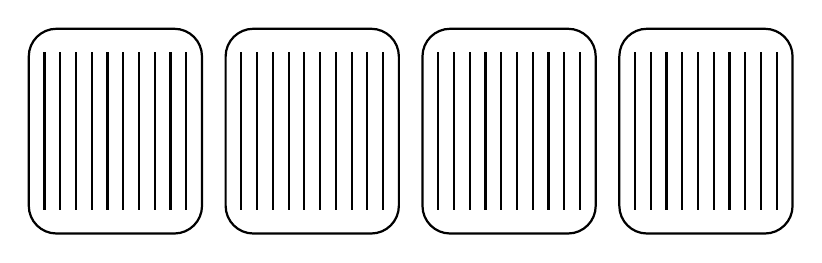
\begin{tikzpicture}
  % Parameters
  \def\stickheight{2}
  \def\stickgap{0.2}
  \def\ovalpad{0.2}
  \def\bundleSpacing{2.5} % narrow spacing

  % Define bundle drawing as a TikZ pic
  \tikzset{
    bundle/.pic={
      % Draw 10 sticks
      \foreach \i in {0,...,9} {
        \draw[thick] (\i*\stickgap,0) -- (\i*\stickgap,\stickheight);
      }
      % Oval around bundle
      \draw[thick, rounded corners=10pt]
        (-\ovalpad, -0.3) rectangle (9*\stickgap+\ovalpad, \stickheight+0.3);
    }
  }

  % Draw 4 bundles
  \foreach \i in {0,...,3} {
    \begin{scope}[shift={(\i*\bundleSpacing,0)}]
      \pic{bundle};
    \end{scope}
  }

\end{tikzpicture}
\end{image}
Now, which number is larger? Since we used the same value for the sticks in both pictures, the larger number will be the one with more total sticks in it. One strategy we could use is to count the sticks. We see that to represent $0.39$ we used $\answer[given]{39}$ sticks, and to represent $0.4$ we used $\answer[given]{40}$ sticks. Since $40 > 39$, we see that $0.4$ is larger than $0.39$.

Alternatively, we could use the idea of one-to-one correspondence to decide which number is larger. We can line up our two pictures by place value. The first three bundles match exactly in both pictures. But then in the picture of $0.4$ we have another bundle while in the picture of $0.39$ we have $9$ loose sticks. We can unbundle the $4$th bundle in $0.4$ and then match up the sticks. After we match $9$ sticks in each picture, we are out of sticks in $0.39$, while we still have a stick left over in $0.4$. This means that $0.4$ is the larger number.

\end{explanation}
\end{question}


\begin{question}
In the previous example, we wrote $0.4$ as $0.40$ and claimed we didn't change anything. Why does this make sense, but it does not make sense to say that $4$ and $40$ are the same?
\begin{freeResponse}
Write your thoughts here. If you aren't sure, this is a great question for office hours!
\end{freeResponse}
\end{question}

Perhaps you remember a rule for comparing decimal numbers that goes something like this. Start by lining up the decimal points. Then move from left to right, comparing the digits as you go. The first number that has a larger digit is the bigger number. For example, if we compare $4292.4873$ to $4285.99485$ we would line up the numbers like this.
\begin{align*}
4292.&4873\\
4285.&99485
\end{align*}
We start on the left side. Both numbers have a $4$ in the thousands place, so we move to the hundreds place. Then, both numbers have a $2$, so we move to the tens place. The top number has a $9$ where the bottom number has an $8$, so the bottom number is the smaller one, or $4285.99485 < 4292.4873$. We hope that you can now see why this rule makes sense in terms of bundled objects. When we line up the decimal points, that's the same as drawing our picture of bundled sticks so that the value of the stick is the same for both numbers. When we start comparing the numbers from the left, we are using the idea of one-to-one correspondence to say whether or not we have the same number of sticks in each place. When we reach a place where we don't have a one-to-one correspondence we can stop because of the structure of the bundling system. No matter what comes after the unequal place value, those sticks and bundles will not be enough to make up a full extra bundle. So the number with a higher value in that place is the larger number, because it will have more total sticks. For instance, in our example, we had a $9$ in the tens place of the larger number, but only an $8$ in the tens place of the smaller number. Even though the smaller number has more digits after the tens place, the $5.99485$ represented in sticks was not enough to complete the $9$th bundle in the tens place. So $4292.4873$ has to have more total sticks. Whenever you are working with someone who is confused about the rules for comparing decimals, it's always a great idea to come back to bundling and draw some pictures.

\begin{question}
Which number is larger: $1.4009$ or $1.42$? Draw a picture in your notes to solve this problem.

\begin{multipleChoice}
\choice{$1.4009$}
\choice[correct]{$1.42$}
\choice{The two numbers are equal}
\choice{We cannot tell from this information}
\end{multipleChoice}
\end{question}


\section{Comparing decimals using paper strips}


Let's see how to use paper strips to compare two decimal numbers. If you've forgotten how to represent decimals using paper strips, don't hesitate to head back to the \link[Decimals]{https://ximera.osu.edu/m4t/elementaryTeachersOne/elementaryReading/Numbers/Decimals} section.

\begin{example}
Use paper strips to show which of $0.083$ and $0.102$ is the larger decimal.

We first need to draw both of these numbers using our paper strips. In this case, let's choose the value of our unit to be one in the tenths place since we don't need any place values to the left of that one. In other words, one full strip will equal $0.1$. When we unbundle that strip, we'll move one place to the right so each smaller strip will equal $0.01$ and then when we unbundle that smaller strip we'll move one place to the right again so each tiny strip will equal $0.001$. Let's draw each of those pieces.

\begin{image}
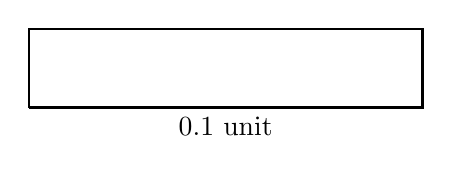
\begin{tikzpicture}
	\draw[thick] (0,0)--(5,0)--(5,1)--(0,1)--(0,0);
	\node[below] at (2.5,0) {$0.1$ unit};
\end{tikzpicture}
\end{image}
\begin{image}
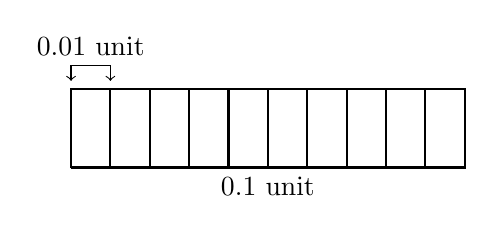
\begin{tikzpicture}
	\draw[thick] (0,0)--(5,0)--(5,1)--(0,1)--(0,0);
	\foreach \x in {0.5, 1, 1.5, 2, 2.5, 3, 3.5, 4, 4.5} \draw[thick] (\x, 0)--(\x, 1);
	\node[below] at (2.5,0) {$0.1$ unit};
	\node[above] at (0.25, 1.3) {$0.01$ unit};
	\draw[<->] (0, 1.1)--(0, 1.3)--(0.5, 1.3)--(0.5, 1.1);
\end{tikzpicture}
\end{image}
\begin{image}
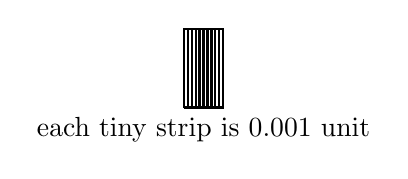
\begin{tikzpicture}
\draw[thick] (0,0)--(0.5,0)--(0.5, 1)--(0,1)--(0,0);
\foreach \x in {0.05, 0.1, 0.15, 0.2, 0.25, 0.3, 0.35, 0.4, 0.45} \draw[thick] (\x, 0)--(\x, 1);
\node[below] at (0.25, 0) {each tiny strip is $0.001$ unit};
\end{tikzpicture}
\end{image}

Now, we assemble our pieces to draw the strips. For $0.083$, we need the following.
\begin{itemize}
	\item $\answer[given]{0}$ of the $0.1$ strips (because there's a zero in the tenths place)
	\item $\answer[given]{8}$ of the $0.01$ strips (because there's an $8$ in the hundredths place)
	\item $\answer[given]{3}$ of the $0.001$ strips (because there's a $3$ in the thousandths place)
\end{itemize}

For $0.102$, we need the following.
\begin{itemize}
	\item $\answer[given]{1}$ of the $0.1$ strips (because there's a one in the tenths place)
	\item $\answer[given]{0}$ of the $0.01$ strips (because there's a zero in the hundredths place)
	\item $\answer[given]{2}$ of the $0.001$ strips (because there's a $2$ in the thousandths place)
\end{itemize}

Now let's draw these two strips, lining them up on their left-hand sides.

\begin{image}
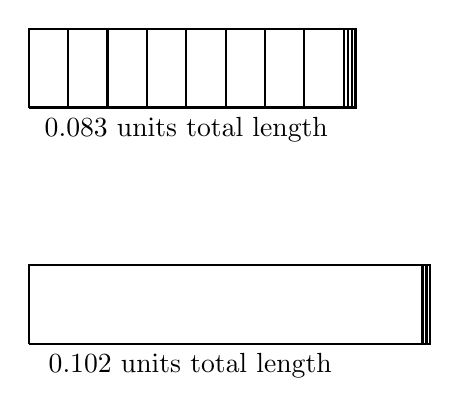
\begin{tikzpicture}
	\draw[thick] (0,0)--(4.15,0)--(4.15,1)--(0,1)--(0,0);
	\foreach \x in {0.5, 1, 1.5, 2, 2.5, 3, 3.5, 4, 4.05, 4.1} \draw[thick] (\x, 0)--(\x,1);
	\node[below] at (2,0) {$0.083$ units total length};
	
	\draw[thick] (0,-3)--(5.1,-3)--(5.1,-2)--(0,-2)--(0,-3);
	\foreach \x in {5, 5.05} \draw[thick] (\x, -3)--(\x,-2);
	\node[below] at (2.05,-3) {$0.102$ units total length};
\end{tikzpicture}
\end{image}

Which number is larger? Since we used the same unit length to build each number, the longer strip is the larger number. In this case, the strip for $0.102$ is longer, and so we see that
\[
0.083 < 0.102.
\]


\end{example}

Remember that when we are comparing numbers, we have to start with the same whole. For paper strips, this means using the same unit size for each of the strips. It's also worthwhile to compare how we can tell which number is larger with bundling and with the paper strips. For bundling, we were looking for the number that had more sticks overall. We could almost think of the paper strips as lining up the sticks in a long horizontal line, and then as long as the sticks are all the same size, the longer strip would also be the one with more sticks. So these ideas make sense together.

\begin{question}
Which number is larger, $3.08$ or $2.86$? Use paper strips to decide.

\begin{multipleChoice}
\choice[correct]{$3.08$}
\choice{$2.86$}
\choice{The two numbers are equal}
\choice{We cannot tell from this information}
\end{multipleChoice}
\end{question}




\section{Comparing decimals with number lines}


It's time for one last example: comparing decimals using a number line.

\begin{example}
Use a number line to decide which of $145.003$ and $145.030$ is the larger number.

Remember that our goal is first to estimate the numbers so that we can draw them on a number line. Since we are going to compare these numbers and want to use the same whole, we want to draw them on the same number line. In other words, we need an estimate that works for both numbers. There are many options, and it's very natural to start with the whole number parts. Let's begin there, marking the left end of our number line as $\answer[given]{145}$ and the right end $\answer[given]{146}$. We'll also start with our line unbundled into tenths in the picture.

\begin{image}
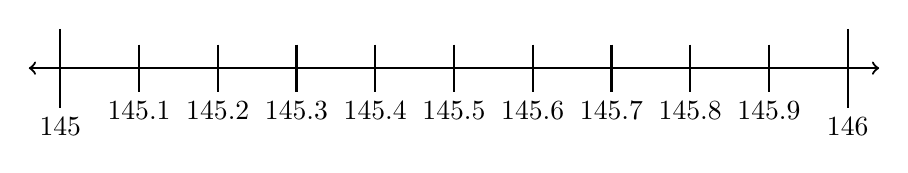
\begin{tikzpicture}
	\draw[thick, <->] (-0.4, 0)--(10.4, 0);
	\foreach \x in {0, 10} \draw[thick] (\x, 0.5)--(\x, -0.5);
	\node[below] at (0, -0.5) {$145$};
	\node[below] at (10, -0.5) {$146$};
	\foreach \y in {1, 2, ..., 9} 
		\draw[thick] (\y, 0.3)--(\y, -0.3);
	\node[below] at (1, -0.3) {$145.1$};
	\node[below] at (2, -0.3) {$145.2$};
	\node[below] at (3, -0.3) {$145.3$};
	\node[below] at (4, -0.3) {$145.4$};
	\node[below] at (5, -0.3) {$145.5$};
	\node[below] at (6, -0.3) {$145.6$};
	\node[below] at (7, -0.3) {$145.7$};
	\node[below] at (8, -0.3) {$145.8$};
	\node[below] at (9, -0.3) {$145.9$};
\end{tikzpicture} \end{image}

Notice that we didn't draw zero and one on this number line, but we can still imagine them way off to the left in this picture because we have a specific location and the length of one unit.  We could use the length of this unit to back up $145$ units along the line, and then we would hit zero. The arrows on the end of the line remind us that the line goes on forever in both directions.

Now, we need to plot our numbers. Both of them are actually between $145$ and $145.1$ because both numbers have a zero in the tenths place. So we could actually start our number line with $145$ and $145.1$ on either end. Let's draw a picture to show that we have zoomed in on that spot.


\begin{image}
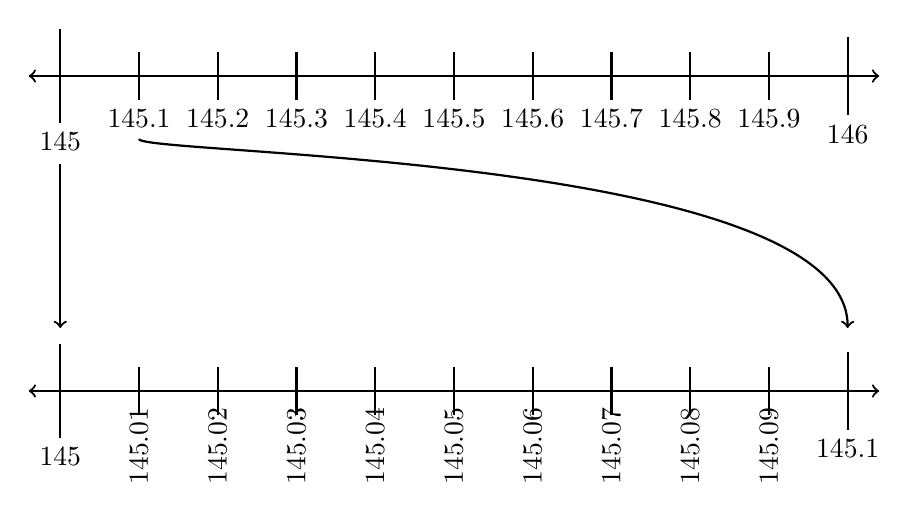
\begin{tikzpicture}
	\draw[thick, <->] (-0.4, 0)--(10.4, 0);
	\draw[thick] (0, 0.6)--(0,-0.6);
	\draw[thick] (10, 0.5)--(10, -0.5);
	\node[below] at (0, -0.6) {$145$};
	\node[below] at (10, -0.5) {$146$};
	\foreach \y in {1, 2, ..., 9} 
		\draw[thick] (\y, 0.3)--(\y, -0.3);
	\node[below] at (1, -0.3) {$145.1$};
	\node[below] at (2, -0.3) {$145.2$};
	\node[below] at (3, -0.3) {$145.3$};
	\node[below] at (4, -0.3) {$145.4$};
	\node[below] at (5, -0.3) {$145.5$};
	\node[below] at (6, -0.3) {$145.6$};
	\node[below] at (7, -0.3) {$145.7$};
	\node[below] at (8, -0.3) {$145.8$};
	\node[below] at (9, -0.3) {$145.9$};
	
	
	\draw[thick, <->] (-0.4, -4)--(10.4, -4);
	\draw[thick] (0, -4.6)--(0, -3.4);
	\draw[thick] (10, -3.5)--(10, -4.5);
		\node[below] at (0, -4.6) {$145$};
		\node[below] at (10, -4.5) {$145.1$};
	\foreach \y in {1, 2, ..., 9} 
		\draw[thick] (\y, -4.3)--(\y, -3.7);
	\node[rotate=90] at (1, -4.7) {$145.01$};
	\node[rotate=90] at (2, -4.7) {$145.02$};
	\node[rotate=90] at (3, -4.7) {$145.03$};
	\node[rotate=90] at (4, -4.7) {$145.04$};
	\node[rotate=90] at (5, -4.7) {$145.05$};
	\node[rotate=90] at (6, -4.7) {$145.06$};
	\node[rotate=90] at (7, -4.7) {$145.07$};
	\node[rotate=90] at (8, -4.7) {$145.08$};
	\node[rotate=90] at (9, -4.7) {$145.09$};
	
	 \draw[->, thick] (0,-1.2) .. controls (0,-1) and (0,-1) .. (0,-3.2);
	  \draw[->, thick] (1,-0.8) .. controls (1,-1) and (10,-1) .. (10,-3.2);	
	
\end{tikzpicture}
\end{image}

One of our numbers is already on the line, since $145.030$ is the same as $145.03$: we don't have to add any thousandths to this number in order to plot it. But our other number, $145.003$, needs three thousandths added on from $145.00 = 145$. Notice this number has no tenths and no hundredths. So we need to add more tick marks between $145$ and $145.01$ by unbundling this part of the number line.

\begin{image}
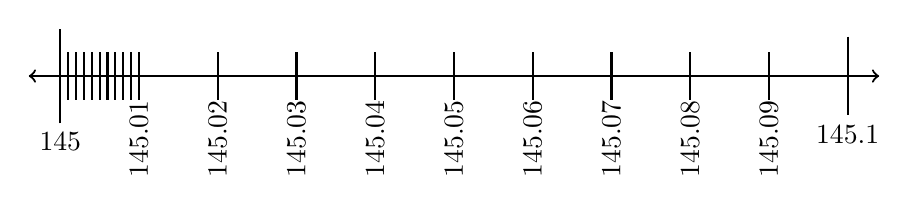
\begin{tikzpicture}
	\draw[thick, <->] (-0.4, -4)--(10.4, -4);
	\draw[thick] (0, -4.6)--(0, -3.4);
	\draw[thick] (10, -3.5)--(10, -4.5);
		\node[below] at (0, -4.6) {$145$};
		\node[below] at (10, -4.5) {$145.1$};
	\foreach \y in {1, 2, ..., 9} 
		\draw[thick] (\y, -4.3)--(\y, -3.7);
	\node[rotate=90] at (1, -4.8) {$145.01$};
	\node[rotate=90] at (2, -4.8) {$145.02$};
	\node[rotate=90] at (3, -4.8) {$145.03$};
	\node[rotate=90] at (4, -4.8) {$145.04$};
	\node[rotate=90] at (5, -4.8) {$145.05$};
	\node[rotate=90] at (6, -4.8) {$145.06$};
	\node[rotate=90] at (7, -4.8) {$145.07$};
	\node[rotate=90] at (8, -4.8) {$145.08$};
	\node[rotate=90] at (9, -4.8) {$145.09$};
	
	\foreach \a in {0.1, 0.2, ..., 0.9} \draw[thick] (\a, -4.3)--(\a, -3.7);
\end{tikzpicture} \end{image}
Each tick mark between $145.00$ and $145.01$ is one thousandth, so the first tick would be marked $145.001$, then $145.002$, and so on. Now, we locate both of our numbers on the line with a dot and label them.


\begin{image}
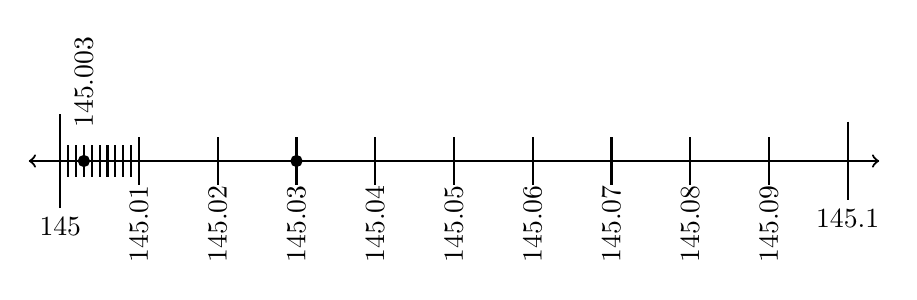
\begin{tikzpicture}
	\draw[thick, <->] (-0.4, -4)--(10.4, -4);
	\draw[thick] (0, -4.6)--(0, -3.4);
	\draw[thick] (10, -3.5)--(10, -4.5);
		\node[below] at (0, -4.6) {$145$};
		\node[below] at (10, -4.5) {$145.1$};
	\foreach \y in {1, 2, ..., 9} 
		\draw[thick] (\y, -4.3)--(\y, -3.7);
	\node[rotate=90] at (1, -4.8) {$145.01$};
	\node[rotate=90] at (2, -4.8) {$145.02$};
	\node[rotate=90] at (3, -4.8) {$145.03$};
	\node[rotate=90] at (4, -4.8) {$145.04$};
	\node[rotate=90] at (5, -4.8) {$145.05$};
	\node[rotate=90] at (6, -4.8) {$145.06$};
	\node[rotate=90] at (7, -4.8) {$145.07$};
	\node[rotate=90] at (8, -4.8) {$145.08$};
	\node[rotate=90] at (9, -4.8) {$145.09$};
	
	\foreach \a in {0.1, 0.2, ..., 0.9} \draw[thick] (\a, -4.2)--(\a, -3.8);
	
	\draw[fill=black] (0.3, -4) circle (2pt);
	\draw[fill=black] (3, -4) circle (2pt);
	\node[rotate=90] at (0.3, -3) {$145.003$};
\end{tikzpicture} \end{image}

Which number is larger? When we draw our number lines in this way, numbers farther to the right of zero are larger, because the position of a number on the line is its length from zero. (Notice that we are just talking about positive numbers for now, but you can think about how you might describe what happens with negative numbers. We'll postpone that for a bit.) A longer distance from zero is a bigger number. Think again about paper strips, and the fact that we said that a longer strip meant a bigger number, and we connected this back to sticks and bundling as well. Each time we move to the right one tick mark on the number line, that's like adding another stick or another bundle or another object of some kind. Using this thinking, we can see that 
\[
145.003 \answer[given]{<} 145.030.
\]
The number $145.030$ is farther to the right on the number line.

\end{example}

As with representing decimals, when you explain how to compare decimal numbers you should first explain how the representation works and why it makes sense. Then, you should explain why your comparison makes sense using these representations. We aren't looking for you to only state the rules!

\begin{question}
Which number is larger, $84.68$ or $84.73$? Use a number line to decide.

\begin{multipleChoice}
\choice{$84.68$}
\choice[correct]{$84.73$}
\choice{The two numbers are equal}
\choice{We cannot tell from this information}
\end{multipleChoice}
\end{question}



\end{document}






